%%%%%%%%%%%%%%%%%%%%%%%%%%%%%%%%%%%%%%%%%%%%%%%%%%%%%%%%%%%%%%%%%%%%%%%
%% Inhaltliches Kapitel (Beispiel)
\section{Beispiel für Inhalte}
\label{sec:content}

Dieses Kapitel ist als Beispiel für die zu erstellenden Inhalte gedacht.



\subsection{Nutzung von Aufzählungen}
    \subsubsection{Einfache Aufzählungen}
        Einfache Aufzählungen erhält man über die \texttt{Itemize}-Umgebung:
        \begin{itemize}
        	\item erster Stichpunkt
        	\item zweiter Stichpunkt
            \begin{itemize}
            	\item erster verschachtelter Stichpunkt
            	\item noch einer
            	\begin{itemize}
            		\item Schachteln auf dritter Ebene
        		\end{itemize}
        	\end{itemize}
        	\item dritter Stichpunkt
        \end{itemize}
        
    \subsubsection{Nummerierte Aufzählungen}
        Aufzählungen lassen sich auch automatisch durchnummerieren mit der
        \texttt{Enumerate}-Umgebung:
        \begin{enumerate}
            \item erster Stichpunkt
            \item zweiter Stichpunkt
            \begin{itemize}
                \item erster verschachtelter Stichpunkt
                \item noch einer
                \begin{itemize}
                    \item Schachteln auf dritter Ebene
                \end{itemize}
            \end{itemize}
            \item dritter Stichpunkt
        \end{enumerate}
        
    \subsubsection{Definitions-Aufzählungen}
        Mit der \texttt{Description}-Umgebung lassen sich Definitions-artige Aufzählungen
        gestalten.
        \begin{description}
            \item[Begriff] und hier die längliche Beschreibung des tollen Begriffs,
            seiner Auswirkungen auf den Geisteszustand des Schreibers und die Folgen für
            den Leser
            \item[B2] noch ein Begriff
        \end{description}
    
    
    
\subsection{Tabellen und Bilder}
    \subsubsection{Einbinden von Abbildungen}
        Einfache Abbildungen lassen sich mit der \texttt{Figure}-Umgebung und dem
        \texttt{includegraphics}-Befehl einbinden:
        \begin{figure}
            \centering
            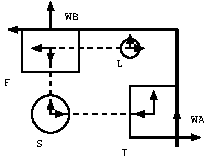
\includegraphics[scale=1.4]{fig/exampleSzene}   
            \caption{Typischer Beispieltext}
            \label{fig:beispielText}
        \end{figure}
            
        Abbildungen mit mehreren Teilabbildungen lassen sich über die
        \texttt{Subfigure}-Umgebung nutzen.
        \begin{figure}
            \centering
            \subfigure[teil 1]{%
                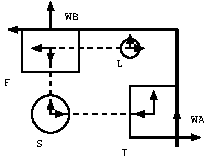
\includegraphics[scale=1]{fig/exampleSzene}
                \label{fig:beispielDepiktionenA}}
            \hfill
            \subfigure[teil 2]{%
                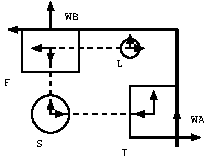
\includegraphics[scale=1]{fig/exampleSzene}
                \label{fig:beispielDepiktionenB}}
            \vfill
            \subfigure[teil 3]{%
                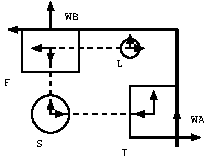
\includegraphics[scale=1]{fig/exampleSzene}
                \label{fig:beispielDepiktionenC}}
            \caption{Zum Beispieltext passende Abbildungen (Depiktionen)}
            \label{fig:beispielDepiktionen}
        \end{figure}
        
        Als Quellen eigenen sich PDF- und JPG-Dateien. Andere Dateien müssen vor der
        Benutzung konvertiert werden.
    
    
    \subsubsection{Tabellen}
        Tabellen gehen in der \texttt{Table}-Umgebung mit Hilfe des \texttt{tabular}-Befehls.
        \begin{table}
            \centering
            \begin{tabular}{l|l||r}
                \multicolumn{2}{l}{zwei Spalten zusammengefasst} & dritte Spalte\\
                Spalte 1 & Spalte 2 & Spalte 3 \\\hline\hline
                Spalte 1 & Spalte 2 & Spalte 3 \\\hline
                Spalte 1 & Spalte 2 & Spalte 3 \\\hline
            \end{tabular}
            \caption{Beispieltabelle}
            \label{tab:beispieltabelle}
        \end{table}
        
        Ansonsten funktioniert die Umgebung änhlich wie die
        \texttt{Figure}-Umgebung.
    
    
    \subsubsection{Quellcode}
        Quellcode lässt sich mit Hilfe des \texttt{Listings}-Paketes einbinden.
        Sinnvollerweise definiert man sich dazu in der Präambel des
        Hauptdokuments eine passende neue \texttt{lstnewenvironment}-Umgebung, die man
        dann einfach nutzen kann und die neben Snytax-Highlighting auch andere
        Dinge wie Rahmen, Zeilennummern, Bildunter- oder überschriften
        etc.~beherrscht.
        
        \begin{figure}
        \centering
        \begin{java}
public class Student {
    private String name;

    public Student(String name) {
        this.name = name; 
    }
    
    public static void main(String[] args) {
        Student s = new Student();
    }
}
        \end{java}
        \caption{Sourcecode für Kram}
        \label{fig:source}
        \end{figure}
        
        
     \subsubsection{Quellcode}
        Algorithmen schreibt man entweder als Pseudocode (über das
        \texttt{Listings}-Paket) oder aber mit Hilfe der \texttt{algorithm}-Umgebung aus
        dem Paket \texttt{algorithm2e}
        
        \begin{center}
        \begin{algorithm}[ht]
        \DontPrintSemicolon
        \LinesNumbered
        \SetKwFunction{init}{init}
        \SetKwFunction{evaluate}{evaluate}
        \SetKwFunction{recombine}{recombine}
        \SetKwFunction{mutate}{mutate}
        \SetKwFunction{select}{select}
        \SetKw{nicht}{not}
        \SetKw{und}{and}
        \Begin{
            $t$ = 0\;
            \init{$P(t)$}\;
            \evaluate{$P(t)$}\;
            \While{\nicht optimal \und \nicht Abbruch}{
                $PP(t) = $ \recombine{$P(t)$}\;
                \mutate{$PP(t)$}\;
                \evaluate{$PP(t)$}\;
                $P(t+1) = $ \select{$PP(t)$, $P(t)$}\;
                $t = t+1$\;
            }
        }
        \caption{Ablauf eines hybriden EA}
        \label{alg:eaHybrid}
        \end{algorithm}
        \end{center}
        

    
\subsection{Referenzierungen}
    \subsubsection{Zitate}
    Zitieren geht mit dem Befehl \texttt{cite}: \cite{Claus98a} bzw. mit den Befehl
    \texttt{citep}: \citep{wagner2009tele}. Als Argument
    benötigt man den Schlüssel für die jeweilige Referenz, so wie er in der
    .bib-Datei hinterlegt ist bzw.~durch Tools wie JabRef generiert wird. 
    
    Wenn man etwas nicht direkt zitieren möchte, aber die Literaturquelle im
    Literaturverzeichnis erscheinen soll, dann nutzt man den Befehl
    \texttt{nocite}.
    
    \subsubsection{Querverweise}
    Den Anker für die Querverweise setzt man mit dem Befehl \texttt{label}.
    Bezugnehmen kann man dann mit Hilfe von \texttt{ref} oder \texttt{pageref},
    wobei ersteres durch die entsprechende Gliederungsnummer (Überschrift,
    Abbildung, Tabelle, \ldots) ersetzt wird und letzteres durch die
    Seitennummer, auf der der Anker für die Referenz gesetzt wurde.
    Beispiel: Abbildung \ref{fig:beispielText} erscheint auf Seite
    \pageref{fig:beispielText}.
    
    
\subsection{Fussnoten}
    Fussnoten setzt man mit Hilfe des Befehls \texttt{footnote}. Dieser folgt
    entweder direkt auf das Wort, welches man mit einer Fussnote versehen möchte
    oder aber auf das Satzendezeichen, wenn man einen ganzen Satz/Absatz meint.
    Beispiel:\footnote{Das ist meine erste Fussnote.}
    
    
\subsection{Mathe}
Für Mathe siehe \href{http://www.ams.org/tex/short-math-guide.html}{{\tt
www.ams.org/tex/short-math-guide.html}}.


    
    
    
